\begin{problem}[问题5.2]一水箱底部有一小孔, 射流的截

\vspace{-2em}
\begin{multicols}{2}
~

面积为$A(x)$, 在小孔处$x=0$, 截面积为$A_0$. 通过不断注水使水箱中水高$h$保持常数, 水箱的横截面远比小孔的大. 设流体是理想, 不可压缩的, 求射流截面积随x的变化规律$A(x)$.
\begin{center}
%\includegraphics[width=0.25\textwidth]{./figures/problem02.pdf}
\usetikzlibrary{%
    decorations.pathreplacing,%
    decorations.pathmorphing,arrows
}
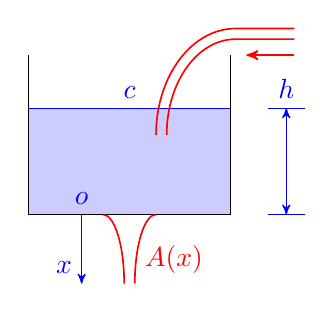
\begin{tikzpicture}[scale=1.35]
\fill[blue!20](-0.25,1)--(-0.25,0)--(1.65,0)--(1.65,1);
\draw[blue](-0.25,1)--(1.65,1) node[midway,above]{$c$};
\draw[semithick](-0.25,1.5)--(-0.25,0)--(1.65,0)--(1.65,1.5);

\draw[semithick,red](0.95,0.75) arc(180:90:0.75 and 1) --(2.25,1.75) (1.05,0.75) arc(180:90:0.65 and 0.9)--(2.25,1.65);
\draw[semithick,red,->,>=stealth'] (2.25,1.5)--(1.8,1.5);

\draw[blue](2,1)--(2.35,1) (2,0)--(2.35,0);

\draw[blue,<->,>=stealth'] (2.175,0)--(2.175,1) node[above]{$h$}; 

\draw[blue,->,>=stealth'] (0.25,0)node[above]{$o$}--(0.25,-0.65) node[above left]{$x$} ; 

\draw[red,semithick](0.45,0) arc(90:0:0.2 and 0.65) (0.95,0) arc(90:180:0.2 and 0.65) node[above right]{$A(x)$};

\end{tikzpicture}

\end{center}
\end{multicols}
\end{problem}

\begin{solution}
\textbf{解:}设水箱的液面为c, 则对$c$, $o$, 及任意射流面A(x)处应用Bernoulli方程
\[
\frac{1}{2}v_c^2 + \frac{p_c}{\rho} - gx_c =
\frac{1}{2}v_o^2 + \frac{p_o}{\rho} - gx_o =
\frac{1}{2}v_x^2 + \frac{p_x}{\rho} - gx
\]
由于$v_c=0$, $p_c = p_o = p_x$, $x_c=-h$,$x_o = 0$,因此上式可化为
\[
gh = \frac{1}{2}v_o^2 = \frac{1}{2}v_x^2 -gx
\]
因此可求得任意射流$x$处的射流速度
\[
v_x = \sqrt{2g(h+x)} , {~~} v_o = \sqrt{2gh}
\]
又因为$A(x)v_x = A_ov_o=A_o\sqrt{2gh}$, 因此可求得射流面积$A(x)$
\[
A(x) = A_o\sqrt{\frac{h}{h+x}}
\]
\end{solution} 
